\documentclass[dvipdfmx]{jsarticle}
\setcounter{section}{1}
\setcounter{subsection}{1}
\usepackage{xr}
\externaldocument{8.1.1}
\usepackage{amsmath,amsfonts,amssymb,array,comment,mathtools,url,docmute}
\usepackage{longtable,booktabs,dcolumn,tabularx,mathtools,multirow,colortbl,xcolor}
\usepackage[dvipdfmx]{graphics}
\usepackage{bmpsize}
\usepackage{amsthm}
\usepackage{enumitem}
\setlistdepth{20}
\renewlist{itemize}{itemize}{20}
\setlist[itemize]{label=•}
\renewlist{enumerate}{enumerate}{20}
\setlist[enumerate]{label=\arabic*.}
\setcounter{MaxMatrixCols}{20}
\setcounter{tocdepth}{3}
\newcommand{\rotin}{\text{\rotatebox[origin=c]{90}{$\in $}}}
\newcommand{\amap}[6]{\text{\raisebox{-0.7cm}{\begin{tikzpicture} 
  \node (a) at (0, 1) {$\textstyle{#2}$};
  \node (b) at (#6, 1) {$\textstyle{#3}$};
  \node (c) at (0, 0) {$\textstyle{#4}$};
  \node (d) at (#6, 0) {$\textstyle{#5}$};
  \node (x) at (0, 0.5) {$\rotin $};
  \node (x) at (#6, 0.5) {$\rotin $};
  \draw[->] (a) to node[xshift=0pt, yshift=7pt] {$\textstyle{\scriptstyle{#1}}$} (b);
  \draw[|->] (c) to node[xshift=0pt, yshift=7pt] {$\textstyle{\scriptstyle{#1}}$} (d);
\end{tikzpicture}}}}
\newcommand{\twomaps}[9]{\text{\raisebox{-0.7cm}{\begin{tikzpicture} 
  \node (a) at (0, 1) {$\textstyle{#3}$};
  \node (b) at (#9, 1) {$\textstyle{#4}$};
  \node (c) at (#9+#9, 1) {$\textstyle{#5}$};
  \node (d) at (0, 0) {$\textstyle{#6}$};
  \node (e) at (#9, 0) {$\textstyle{#7}$};
  \node (f) at (#9+#9, 0) {$\textstyle{#8}$};
  \node (x) at (0, 0.5) {$\rotin $};
  \node (x) at (#9, 0.5) {$\rotin $};
  \node (x) at (#9+#9, 0.5) {$\rotin $};
  \draw[->] (a) to node[xshift=0pt, yshift=7pt] {$\textstyle{\scriptstyle{#1}}$} (b);
  \draw[|->] (d) to node[xshift=0pt, yshift=7pt] {$\textstyle{\scriptstyle{#2}}$} (e);
  \draw[->] (b) to node[xshift=0pt, yshift=7pt] {$\textstyle{\scriptstyle{#1}}$} (c);
  \draw[|->] (e) to node[xshift=0pt, yshift=7pt] {$\textstyle{\scriptstyle{#2}}$} (f);
\end{tikzpicture}}}}
\renewcommand{\thesection}{第\arabic{section}部}
\renewcommand{\thesubsection}{\arabic{section}.\arabic{subsection}}
\renewcommand{\thesubsubsection}{\arabic{section}.\arabic{subsection}.\arabic{subsubsection}}
\everymath{\displaystyle}
\allowdisplaybreaks[4]
\usepackage{vtable}
\theoremstyle{definition}
\newtheorem{thm}{定理}[subsection]
\newtheorem*{thm*}{定理}
\newtheorem{dfn}{定義}[subsection]
\newtheorem*{dfn*}{定義}
\newtheorem{axs}[dfn]{公理}
\newtheorem*{axs*}{公理}
\renewcommand{\headfont}{\bfseries}
\makeatletter
  \renewcommand{\section}{%
    \@startsection{section}{1}{\z@}%
    {\Cvs}{\Cvs}%
    {\normalfont\huge\headfont\raggedright}}
\makeatother
\makeatletter
  \renewcommand{\subsection}{%
    \@startsection{subsection}{2}{\z@}%
    {0.5\Cvs}{0.5\Cvs}%
    {\normalfont\LARGE\headfont\raggedright}}
\makeatother
\makeatletter
  \renewcommand{\subsubsection}{%
    \@startsection{subsubsection}{3}{\z@}%
    {0.4\Cvs}{0.4\Cvs}%
    {\normalfont\Large\headfont\raggedright}}
\makeatother
\makeatletter
\renewenvironment{proof}[1][\proofname]{\par
  \pushQED{\qed}%
  \normalfont \topsep6\p@\@plus6\p@\relax
  \trivlist
  \item\relax
  {
  #1\@addpunct{.}}\hspace\labelsep\ignorespaces
}{%
  \popQED\endtrivlist\@endpefalse
}
\makeatother
\renewcommand{\proofname}{\textbf{証明}}
\usepackage{tikz,graphics}
\usepackage[dvipdfmx]{hyperref}
\usepackage{pxjahyper}
\hypersetup{
 setpagesize=false,
 bookmarks=true,
 bookmarksdepth=tocdepth,
 bookmarksnumbered=true,
 colorlinks=false,
 pdftitle={},
 pdfsubject={},
 pdfauthor={},
 pdfkeywords={}}
\begin{document}
%\hypertarget{ux958bux57fa}{%
\subsection{開基}%\label{ux958bux57fa}}
%\hypertarget{ux4f4dux76f8ux306eux5f37ux5f31}{%
\subsubsection{位相の強弱}%\label{ux4f4dux76f8ux306eux5f37ux5f31}}
\begin{dfn}
1つの空集合でない集合$S$における2つの位相たち$\mathfrak{O}$、$\mathfrak{P}$が$\mathfrak{O \subseteq P}$を満たすとき、その位相$\mathfrak{O}$はその位相$\mathfrak{P}$より弱い、その位相$\mathfrak{P}$はその位相$\mathfrak{O}$より強いなどという。以上のように定義されることができるその集合$S$における位相たち全体の集合を$\mathcal{T}(S)$としよう。
\end{dfn}
\begin{thm}\label{8.1.2.1}
この組$\left( \mathcal{T}(S), \subseteq \right)$は明らかに順序集合をなす。
\end{thm}\par
ただし、全順序集合ではないことを注意されたい。
\begin{proof} 順序集合の公理にあてはめれば、直ちに示される。
\end{proof}
\begin{thm}\label{8.1.2.2} また、明らかに次式が成り立つ。
\begin{align*}
\min{\mathcal{T}(S)} &= \mathfrak{O}_{*} = \left\{ \emptyset,S \right\}\\
\max{\mathcal{T}(S)} &= \mathfrak{O}^{*} = \mathfrak{P}(S)
\end{align*}
\end{thm}
\begin{proof}
位相の公理より任意の位相$\mathfrak{O}$はその集合$\mathfrak{P}(S)$の部分集合であるかつ、$\mathfrak{O \subset}\left\{ \emptyset,S \right\}$なる位相$\mathfrak{O}$が存在すれば、これは位相の公理を満たさない。背理法により任意の位相$\mathfrak{O}$に対し、$\left\{ \emptyset,S \right\}\subseteq \mathfrak{O}$が成り立つ。これにより、示すべきことが示される。
\end{proof}
\begin{thm}\label{8.1.2.3}
それらの位相たち$\mathfrak{O}$、$\mathfrak{P}$から定まる閉集合系たちをそれぞれ$\mathfrak{A}$、$\mathfrak{B}$、全近傍系をそれぞれ$\mathbf{V}(a)$、$\mathbf{W}(a)$とおくと、次のことは同値である。
\begin{itemize}
\item
  $\mathfrak{O \subseteq P}$が成り立つ。
\item
  $\mathfrak{A \subseteq B}$が成り立つ。
\item
  $\forall a \in S$に対し、$\mathbf{V}(a) \subseteq \mathbf{W}(a)$が成り立つ。
\end{itemize}
\end{thm}
\begin{proof}
1つの空集合でない集合$S$における2つの位相たち$\mathfrak{O}$、$\mathfrak{P}$が$\mathfrak{O \subseteq P}$を満たすならそのときに限り、$\forall O \in \mathfrak{O}$に対し、$O \in \mathfrak{O}$が成り立つなら、$O \in \mathfrak{P}$が成り立つ。ここで、その集合$O$が$S \setminus A$と書き換えられると、それらの位相たち$\mathfrak{O}$、$\mathfrak{P}$から定まる閉集合系たちをそれぞれ$\mathfrak{A}$、$\mathfrak{B}$とおいて、$\forall A \in \mathfrak{A}$に対し、$A \in \mathfrak{A}$が成り立つなら、$A \in \mathfrak{B}$が成り立つので、これが成り立つならそのときに限り、$\mathfrak{A \subseteq B}$が成り立つ。以上より、次のことは同値であることが示された。
\begin{itemize}
\item
  $\mathfrak{O \subseteq P}$が成り立つ。
\item
  $\mathfrak{A \subseteq B}$が成り立つ。
\end{itemize}\par
また、それらの位相たち$\mathfrak{O}$、$\mathfrak{P}$が$\mathfrak{O \subseteq P}$を満たすとき、$\forall a \in S$に対し、全近傍系をそれぞれ$\mathbf{V}(a)$、$\mathbf{W}(a)$とおくと、$V \in \mathbf{V}(a)$が成り立つなら、定義より明らかに$\exists O \in \mathfrak{O}$に対し、$a \in O$かつ$O \subseteq V$が成り立ち、$\mathfrak{O \subseteq P}$が成り立つことに注意すれば、$O \in \mathfrak{P}$が成り立ち、これにより、$V \in \mathbf{W}(a)$が成り立つ。ゆえに、$\mathbf{V}(a) \subseteq \mathbf{W}(a)$が得られる。逆に、$\forall a \in S$に対し、$\mathbf{V}(a) \subseteq \mathbf{W}(a)$が成り立つとき、$\forall O \in \mathfrak{O}$に対し、$O \in \mathfrak{O}$が成り立つならそのときに限り、$\forall a \in O$に対し、$a \in {\mathrm{int}}O$が成り立つので、$a \in O$が成り立つなら、$O \in \mathbf{V}(a)$が成り立ち、したがって、$O \in \mathbf{W}(a)$が成り立つ。これにより、$O \in \mathfrak{P}$が成り立つ。以上より、$\mathfrak{O \subseteq P}$が得られた。以上の議論により、次のことは同値であることが示された。
\begin{itemize}
\item
  $\mathfrak{O \subseteq P}$が成り立つ。
\item
  $\forall a \in S$に対し、$\mathbf{V}(a) \subseteq \mathbf{W}(a)$が成り立つ。
\end{itemize}
\end{proof}
\begin{thm}\label{8.1.2.4}
その集合$\mathcal{T}(S)$の任意の元の族$\left\{ \mathfrak{O}_{\lambda} \right\}_{\lambda \in \varLambda}$が与えられたとき、その集合$\left\{ \mathfrak{O}_{\lambda} \right\}_{\lambda \in \varLambda}$の上限$\sup\left\{ \mathfrak{O}_{\lambda} \right\}_{\lambda \in \varLambda}と下限\inf\left\{ \mathfrak{O}_{\lambda} \right\}_{\lambda \in \varLambda}がその集合\mathcal{T}(S)$に存在する。しかも、次式が成り立つ。
\begin{align*}
\sup\left\{ \mathfrak{O}_{\lambda} \right\}_{\lambda \in \varLambda} &= \bigcap_{\scriptsize \begin{matrix}
\mathfrak{O \in}\mathcal{T}(S) \\
\bigcup_{\lambda \in \varLambda} \mathfrak{O}_{\lambda}\subseteq \mathfrak{O} \\
\end{matrix}} \mathfrak{O}\\
\inf\left\{ \mathfrak{O}_{\lambda} \right\}_{\lambda \in \varLambda} &= \bigcap_{\lambda \in \varLambda} \mathfrak{O}_{\lambda}
\end{align*}
\end{thm}\par
ここで、その集合$\bigcup_{\lambda \in \varLambda} \mathfrak{O}_{\lambda}$は必ずしもその集合$S$における位相となるとは限らないことに注意されたい。例えば、$S = \left\{ a,b,c \right\}$、$\mathfrak{O} = \left\{ \emptyset,\left\{ a \right\},S \right\}$、$\mathfrak{P} = \left\{ \emptyset,\left\{ b \right\},S \right\}$が与えられたとき、それらの集合たち$\mathfrak{O}$、$\mathfrak{P}$は位相となるが、$\left\{ a \right\} \cup \left\{ b \right\} \notin \mathfrak{O} \cup \mathfrak{P}$が成り立つので、その集合$\mathfrak{O \cup P}$は位相ではない。
\begin{proof}
その集合$S$における位相たち全体の集合$\mathcal{T}(S)$の任意の元の族$\left\{ \mathfrak{O}_{\lambda} \right\}_{\lambda \in \varLambda}$が与えられたとき、明らかに$\forall\lambda \in \varLambda$に対し、$\mathfrak{O}_{\lambda}\subseteq \mathfrak{P}(S)$が成り立つので、順序集合$\left( \left\{ \mathfrak{O}_{\lambda} \right\}_{\lambda \in \varLambda}, \subseteq \right)$は上に有界であり、その順序集合$\left( \left\{ \mathfrak{O}_{\lambda} \right\}_{\lambda \in \varLambda}, \subseteq \right)$の上界全体の集合を$U\left( \left\{ \mathfrak{O}_{\lambda} \right\}_{\lambda \in \varLambda} \right)$とおくと、$\mathfrak{\forall O \in}U\left( \left\{ \mathfrak{O}_{\lambda} \right\}_{\lambda \in \varLambda} \right)\forall\lambda \in \varLambda$に対し、$\mathfrak{O}_{\lambda}\subseteq \mathfrak{O}$が成り立つことになり、これが成り立つならそのときに限り、$\mathfrak{O \in}\mathcal{T}(S)$かつ$\bigcup_{\lambda \in \varLambda} \mathfrak{O}_{\lambda}\subseteq \mathfrak{O}$が成り立つ。ここで、$\mathfrak{\forall O \in}U\left( \left\{ \mathfrak{O}_{\lambda} \right\}_{\lambda \in \varLambda} \right)$に対し、$\bigcap_{\scriptsize \begin{matrix}
\mathfrak{O \in}U\left( \left\{ \mathfrak{O}_{\lambda} \right\}_{\lambda \in \varLambda} \right) \\
\end{matrix}} \mathfrak{O}\subseteq \mathfrak{O}$が成り立つので、上限の定義と上記の議論により$\sup\left\{ \mathfrak{O}_{\lambda} \right\}_{\lambda \in \varLambda} = \bigcap_{\scriptsize \begin{matrix}
\mathfrak{O \in}\mathcal{T}(S) \\
\bigcup_{\lambda \in \varLambda} \mathfrak{O}_{\lambda}\subseteq \mathfrak{O} \\
\end{matrix}} \mathfrak{O}$が成り立つ。さらに、$\mathfrak{\forall O \in}U\left( \left\{ \mathfrak{O}_{\lambda} \right\}_{\lambda \in \varLambda} \right)$に対し、$S,\emptyset \in \mathfrak{O}$が成り立つので、$S,\emptyset \in \bigcap_{\scriptsize \begin{matrix}
\mathfrak{O \in}U\left( \left\{ \mathfrak{O}_{\lambda} \right\}_{\lambda \in \varLambda} \right) \\
\end{matrix}} \mathfrak{O}$が成り立つかつ、任意の添数集合$M$に対し、$\forall\mu \in M$に対し、$O_{\mu} \in \bigcap_{\scriptsize \begin{matrix}
\mathfrak{O \in}U\left( \left\{ \mathfrak{O}_{\lambda} \right\}_{\lambda \in \varLambda} \right) \\
\end{matrix}} \mathfrak{O}$が成り立つなら、$\mathfrak{\forall O \in}U\left( \left\{ \mathfrak{O}_{\lambda} \right\}_{\lambda \in \varLambda} \right)$に対し、$O_{\mu}\in \mathfrak{O}$が成り立ち$\bigcup_{\mu \in M} O_{\mu}\in \mathfrak{O}$が成り立つので、$\bigcup_{\mu \in M} O_{\mu} \in \bigcap_{\scriptsize \begin{matrix}
\mathfrak{O \in}U\left( \left\{ \mathfrak{O}_{\lambda} \right\}_{\lambda \in \varLambda} \right) \\
\end{matrix}} \mathfrak{O}$が成り立つかつ、$\forall O,P \in \bigcap_{\scriptsize \begin{matrix}
\mathfrak{O \in}U\left( \left\{ \mathfrak{O}_{\lambda} \right\}_{\lambda \in \varLambda} \right) \\
\end{matrix}} \mathfrak{O}$に対し、$\mathfrak{\forall O \in}U\left( \left\{ \mathfrak{O}_{\lambda} \right\}_{\lambda \in \varLambda} \right)$に対し、$O,P \in \mathfrak{O}$が成り立ち$O \cap P \in \mathfrak{O}$が成り立つので、$O \cap P \in \bigcap_{\scriptsize \begin{matrix}
\mathfrak{O \in}U\left( \left\{ \mathfrak{O}_{\lambda} \right\}_{\lambda \in \varLambda} \right) \\
\end{matrix}} \mathfrak{O}$が成り立つ。以上より、その集合$\bigcap_{\scriptsize \begin{matrix}
\mathfrak{O \in}U\left( \left\{ \mathfrak{O}_{\lambda} \right\}_{\lambda \in \varLambda} \right) \\
\end{matrix}} \mathfrak{O}$は位相であり、したがって、$\bigcap_{\scriptsize \begin{matrix}
\mathfrak{O \in}\mathcal{T}(S) \\
\bigcup_{\lambda \in \varLambda} \mathfrak{O}_{\lambda}\subseteq \mathfrak{O} \\
\end{matrix}} \mathfrak{O}\in \mathcal{T}(S)$が成り立つ。\par
また、明らかに$\forall\lambda \in \varLambda$に対し、$\bigcap_{\lambda \in \varLambda} \mathfrak{O}_{\lambda} \subseteq \mathfrak{O}_{\lambda}$が成り立つので、その順序集合$\left( \left\{ \mathfrak{O}_{\lambda} \right\}_{\lambda \in \varLambda}, \subseteq \right)$は下に有界であり、その順序集合$\left( \left\{ \mathfrak{O}_{\lambda} \right\}_{\lambda \in \varLambda}, \subseteq \right)$の下界全体の集合を$L\left( \left\{ \mathfrak{O}_{\lambda} \right\}_{\lambda \in \varLambda} \right)$とおくと、$\mathfrak{\forall O \in}L\left( \left\{ \mathfrak{O}_{\lambda} \right\}_{\lambda \in \varLambda} \right)$に対し、$\mathfrak{O \subseteq}\bigcap_{\lambda \in \varLambda} \mathfrak{O}_{\lambda}$が成り立つので、下限の定義より$\inf\left\{ \mathfrak{O}_{\lambda} \right\}_{\lambda \in \varLambda} = \bigcap_{\lambda \in \varLambda} \mathfrak{O}_{\lambda}$が成り立つ。さらに、$\forall\lambda \in \varLambda$に対し、$S,\emptyset \in \mathfrak{O}_{\lambda}$が成り立つので、$S,\emptyset \in \bigcap_{\scriptsize \begin{matrix}
\mathfrak{O \in}U\left( \left\{ \mathfrak{O}_{\lambda} \right\}_{\lambda \in \varLambda} \right) \\
\end{matrix}} \mathfrak{O}$が成り立つかつ、任意の添数集合$M$に対し、$\forall\mu \in M$に対し、$O_{\mu} \in \bigcap_{\lambda \in \varLambda} \mathfrak{O}_{\lambda}$が成り立つなら、$\forall\lambda \in \varLambda$に対し、$O_{\mu} \in \mathfrak{O}_{\lambda}$が成り立ち$\bigcup_{\mu \in M} O_{\mu} \in \mathfrak{O}_{\lambda}$が成り立つので、$\bigcup_{\mu \in M} O_{\mu} \in \bigcap_{\lambda \in \varLambda} \mathfrak{O}_{\lambda}$が成り立つかつ、$\forall O,P \in \bigcap_{\lambda \in \varLambda} \mathfrak{O}_{\lambda}$に対し、$\forall\lambda \in \varLambda$に対し、$O,P \in \mathfrak{O}_{\lambda}$が成り立ち$O \cap P \in \mathfrak{O}_{\lambda}$が成り立つので、$O \cap P \in \bigcap_{\lambda \in \varLambda} \mathfrak{O}_{\lambda}$が成り立つ。以上より、その集合$\bigcap_{\lambda \in \varLambda} \mathfrak{O}_{\lambda}$は位相であり、したがって、$\bigcap_{\lambda \in \varLambda} \mathfrak{O}_{\lambda}\in \mathcal{T}(S)$が成り立つ。
\end{proof}
%\hypertarget{ux4f4dux76f8ux306eux751fux6210}{%
\subsubsection{位相の生成}%\label{ux4f4dux76f8ux306eux751fux6210}}
\begin{dfn}
$\mathfrak{M \in P}\left( \mathfrak{P}(S) \right)$なる集合$\mathfrak{M}$が与えられたとき、上記の議論によりその集合$S$における位相全体の集合を$\mathcal{T}(S)$とおいて、$\mathfrak{M \subseteq O}$なるその集合$S$における位相$\mathfrak{O}$全体の集合$\mathcal{T}'$の下限$\inf\mathcal{T}'$が存在するのであった。これを$\mathfrak{O}\left( \mathfrak{M} \right)$とおくと、下限の定義より、$\mathfrak{M \subseteq O}$なる位相の中でその位相$\mathfrak{O}\left( \mathfrak{M} \right)$が最も弱い。この位相$\mathfrak{O}\left( \mathfrak{M} \right)$をその集合$\mathfrak{M}$で生成される位相という。明らかに、$\mathfrak{O}\left( \mathfrak{O}\left( \mathfrak{M} \right) \right) = \mathfrak{O}\left( \mathfrak{M} \right)$が成り立つし、$\mathfrak{M}\in \mathcal{T}(S)$が成り立つなら、$\mathfrak{O}\left( \mathfrak{M} \right) = \mathfrak{M}$が成り立つ。
\end{dfn}
\begin{thm}\label{8.1.2.5}
$\mathfrak{\forall M \in P}\left( \mathfrak{P}(S) \right)$に対し、その位相$\mathfrak{O}\left( \mathfrak{M} \right)$は、有限集合である添数集合$\varLambda$によって添数づけられたその集合$\mathfrak{M}$の元の族$\left\{ A_{\lambda} \right\}_{\lambda \in \varLambda}$の積集合全体の集合を$\mathfrak{M}_{0}$として、任意の添数集合$M$によって添数づけられたその集合$\mathfrak{M}_{0}$の元の族$\left\{ B_{\mu} \right\}_{\mu \in M}$の和集合全体の集合に等しい、即ち、集合$\mathfrak{M}_{0}$が次式のように定義されると、
\begin{align*}
\mathfrak{M}_{0} = \left\{ \bigcap_{\scriptsize \begin{matrix}
\lambda \in \varLambda \\
\end{matrix}} A_{\lambda}\in \mathfrak{P}(S) \middle| {\#}\varLambda < \aleph_{0},\ \ \forall\lambda \in \varLambda\left[ A_{\lambda}\in \mathfrak{M} \right] \right\}
\end{align*}
次式が成り立つ。
\begin{align*}
\mathfrak{O}\left( \mathfrak{M} \right) = \left\{ \bigcup_{\mu \in M} B_{\mu}\in \mathfrak{P}(S) \middle| \forall\mu \in M\left[ B_{\mu} \in \mathfrak{M}_{0} \right] \right\}
\end{align*}
\end{thm}
\begin{proof}
$\mathfrak{\forall M \in P}\left( \mathfrak{P}(S) \right)$に対し、次式のように有限集合である添数集合$\varLambda$によって添数づけられたその集合$\mathfrak{M}$の元の族$\left\{ A_{\lambda} \right\}_{\lambda \in \varLambda}$の積集合全体の集合を$\mathfrak{M}_{0}$として、
\begin{align*}
\mathfrak{M}_{0} = \left\{ \bigcap_{\scriptsize \begin{matrix}
\lambda \in \varLambda \\
\end{matrix}} A_{\lambda}\in \mathfrak{P}(S) \middle| {\#}\varLambda < \aleph_{0},\ \ \forall\lambda \in \varLambda\left[ A_{\lambda}\in \mathfrak{M} \right] \right\}
\end{align*}
$\varLambda = \emptyset$のとき、$\bigcap_{\scriptsize \begin{matrix}
\lambda \in \varLambda \\
\end{matrix}} A_{\lambda} = S$が成り立つとする。次に、任意の添数集合$M$によって添数づけられたその集合$\mathfrak{M}_{0}$の元の族$\left\{ B_{\mu} \right\}_{\mu \in M}$の和集合全体の集合を$\widetilde{\mathfrak{M}}$として、
\begin{align*}
\widetilde{\mathfrak{M}} = \left\{ \bigcup_{\mu \in M} B_{\mu}\in \mathfrak{P}(S) \middle| \forall\mu \in M\left[ B_{\mu} \in \mathfrak{M}_{0} \right] \right\}
\end{align*}
$M = \emptyset$のとき、$\bigcup_{\mu \in M} B_{\mu} = \emptyset$が成り立つとする。\par
このとき、$\forall A \in \mathfrak{M}$に対し、$A \in \mathfrak{M}$が成り立つなら、$\bigcap_{} \left\{ A \right\} = A \in \mathfrak{M}$が成り立つので、$\mathfrak{M \subseteq}\mathfrak{M}_{0}$が成り立つかつ、$\forall\mu \in M$に対し、$B_{\mu} \in \mathfrak{M}_{0}$が成り立つことにより$\bigcup_{\mu \in M} B_{\mu} \in \mathfrak{M}_{0}$が成り立ち、$\mathfrak{M}_{0} \subseteq \widetilde{\mathfrak{M}}$が成り立つので、$\mathfrak{M \subseteq}\mathfrak{M}_{0} \subseteq \widetilde{\mathfrak{M}}$が成り立つ。\par
これにより、$\emptyset \in \widetilde{\mathfrak{M}}$が成り立つかつ、$S \in \mathfrak{M}_{0}$が成り立つので、$\emptyset,S \in \widetilde{\mathfrak{M}}$が成り立つ。また、任意の添数集合$N$によって添数づけられたその集合$\widetilde{\mathfrak{M}}$の任意の元の族$\left\{ O_{\nu} \right\}_{\nu \in N}$が与えられたとき、その集合$\widetilde{\mathfrak{M}}$の定義より任意の添数集合たち$M_{\nu}$を用いて、$\forall\nu \in N$に対し、$B_{\mu_{\nu}} \in \mathfrak{M}_{0}$なる集合たち$B_{\mu_{\nu}}$を用いて、$O_{\nu} = \bigcup_{\mu_{\nu} \in M_{\nu}} B_{\mu_{\nu}}$と書かれることができる。したがって、次のようになり、
\begin{align*}
\bigcup_{\nu \in N} O_{\nu} = \bigcup_{\nu \in N} {\bigcup_{\mu_{\nu} \in M_{\nu}} B_{\mu_{\nu}}} = \bigcup_{\forall\nu \in N\left[ \mu_{\nu} \in M_{\nu} \right]} B_{\mu_{\nu}}
\end{align*}
$\forall\nu \in N\forall\mu_{\nu} \in M_{\nu}$に対し、${B_{\nu}}_{\mu_{\nu}} \in \mathfrak{M}_{0}$が成り立つので、$\bigcup_{\forall\nu \in N\left[ \mu_{\nu} \in M_{\nu} \right]} B_{\mu_{\nu}} \in \widetilde{\mathfrak{M}}$が成り立ち$\bigcup_{\nu \in N} O_{\nu} \in \widetilde{\mathfrak{M}}$が成り立つ。$\forall O,P \in \widetilde{\mathfrak{M}}$に対し、その集合$\widetilde{\mathfrak{M}}$の定義より任意の添数集合たち$M_{O}$、$M_{P}$を用いて、$B_{\mu} \in \mathfrak{M}_{0}$なる集合たち$B_{\mu}$を用いて、$O = \bigcup_{\mu \in M_{O}} B_{\mu}$、$P = \bigcup_{\mu \in M_{P}} B_{\mu}$と書かれることができる。したがって、次のようになり、
\begin{align*}
O \cap P &= \bigcup_{\mu \in M_{O}} B_{\mu} \cap \bigcup_{\mu \in M_{P}} B_{\mu}\\
&= \bigcup_{\scriptsize \begin{matrix}
\mu_{O} \in M_{O},\mu_{P} \in M_{P} \\
\end{matrix}} \left( B_{\mu_{O}} \cap B_{\mu_{P}} \right)
\end{align*}
その集合$\mathfrak{M}_{0}$の定義より有限集合である添数集合たち$\varLambda_{\mu_{O}}$、$\varLambda_{\mu_{P}}$を用いて、$A_{\lambda\mu_{O}},A_{\lambda\mu_{P}}\in \mathfrak{M}$なる集合たち$A_{\lambda\mu_{O}}$、$A_{\lambda\mu_{P}}$を用いて、$B_{\mu_{O}} = \bigcap_{\scriptsize \begin{matrix}
\lambda\mu_{O} \in \varLambda_{\mu_{O}} \\
\end{matrix}} A_{\lambda\mu_{O}}$、$B_{\mu_{P}} = \bigcap_{\scriptsize \begin{matrix}
\lambda\mu_{P} \in \varLambda_{\mu_{P}} \\
\end{matrix}} A_{\lambda\mu_{P}}$と書かれることができる。したがって、次のようになる。
\begin{align*}
B_{\mu_{O}} \cap B_{\mu_{P}} = \bigcap_{\scriptsize \begin{matrix}
\lambda\mu_{O} \in \varLambda_{\mu_{O}} \\
\end{matrix}} A_{\lambda\mu_{O}} \cap \bigcap_{\scriptsize \begin{matrix}
\lambda\mu_{P} \in \varLambda_{\mu_{P}} \\
\end{matrix}} A_{\lambda\mu_{P}}
\end{align*}
これにより、$B_{\mu_{O}} \cap B_{\mu_{P}} \in \mathfrak{M}_{0}$が成り立つので、$O \cap P \in \widetilde{\mathfrak{M}}$が成り立つ。以上より、その集合$\widetilde{\mathfrak{M}}$はその集合$S$における位相となる。\par
一方で、$\mathfrak{\forall O \in}\mathcal{T}(S)$に対し、$\mathfrak{M \subseteq O}$が成り立つとき、$\forall A \in \mathfrak{M}_{0}$に対し、$A \in \mathfrak{M}_{0}$が成り立つなら、有限集合である添数集合$\varLambda$によって添数づけられたその集合$\mathfrak{M}$の元の族$\left\{ A_{\lambda} \right\}_{\lambda \in \varLambda}$の積集合$\bigcap_{\scriptsize \begin{matrix}
\lambda \in \varLambda \\
\end{matrix}} A_{\lambda}$を用いて$A = \bigcap_{\scriptsize \begin{matrix}
\lambda \in \varLambda \\
\end{matrix}} A_{\lambda}$と書かれることができる。ここで、$\forall\lambda \in \varLambda$に対し、$A_{\lambda}\in \mathfrak{M \subseteq}\mathfrak{O}$が成り立つかつ、位相の定義より$\bigcap_{\scriptsize \begin{matrix}
\lambda \in \varLambda \\
\end{matrix}} A_{\lambda}\in \mathfrak{O}$が成り立つ。したがって、$A \in \mathfrak{O}$が成り立ち$\mathfrak{M}_{0}\subseteq \mathfrak{O}$が成り立つ。さらに、$\forall B \in \widetilde{\mathfrak{M}}$に対し、$B \in \widetilde{\mathfrak{M}}$が成り立つなら、任意の添数集合$M$によって添数づけられたその集合$\mathfrak{M}_{0}$の元の族$\left\{ B_{\mu} \right\}_{\mu \in M}$の和集合$\bigcup_{\mu \in M} B_{\mu}$を用いて$B = \bigcup_{\mu \in M} B_{\mu}$と書かれることができる。ここで、$\forall\mu \in M$に対し、$B_{\mu} \in \mathfrak{M}_{0}\subseteq \mathfrak{O}$が成り立つかつ、位相の定義より$\bigcup_{\mu \in M} B_{\mu}\in \mathfrak{O}$が成り立つ。したがって、$B \in \mathfrak{O}$が成り立ち$\widetilde{\mathfrak{M}}\subseteq \mathfrak{O}$が成り立つ。これにより、$\mathfrak{M \subseteq O}$なる位相の中でその位相$\widetilde{\mathfrak{M}}$が最も弱いことになり$\widetilde{\mathfrak{M}} = \mathfrak{O}\left( \mathfrak{M} \right)$が成り立つ。
\end{proof}
%\hypertarget{ux958bux57fa-1}{%
\subsubsection{開基}%\label{ux958bux57fa-1}}
\begin{dfn}
その集合$S$における1つの位相$\mathfrak{O}$が与えられたとき、$\mathfrak{\exists M \in P}\left( \mathfrak{O} \right)$に対し、$\mathfrak{O} = \mathfrak{O}\left( \mathfrak{M} \right)$となるようなその集合$\mathfrak{M}$をその位相空間$\left( S,\mathfrak{O} \right)$の準開基、準基底という。\par
さらに、$\mathfrak{\exists B \in P}\left( \mathfrak{O} \right)\forall O \in \mathfrak{O}$に対し、その集合$O$は添数集合$\varLambda$によって添数づけられたその集合$\mathfrak{B}$の元の族$\left\{ W_{\lambda} \right\}_{\lambda \in \varLambda}$の和集合であるようなその集合$\mathfrak{B}$をその位相空間$\left( S,\mathfrak{O} \right)$の開基、基底という。
\end{dfn}\par
もちろん、その位相空間$\left( S,\mathfrak{O} \right)$の準開基、開基は一意的に存在するというわけではない。
\begin{thm}\label{8.1.2.6}
位相空間$\left( S,\mathfrak{O} \right)$の任意の開基$\mathfrak{B}$はその位相空間$\left( S,\mathfrak{O} \right)$の準開基でもあり$\mathfrak{O} = \mathfrak{O}\left( \mathfrak{B} \right)$が成り立つ。
\end{thm}
\begin{proof}
位相空間$\left( S,\mathfrak{O} \right)$が与えられたとき、その位相空間$\left( S,\mathfrak{O} \right)$の任意の開基$\mathfrak{B}$は、$\forall O \in \mathfrak{O}$に対し、その集合$O$は添数集合$\varLambda$によって添数づけられたその集合$\mathfrak{B}$の元の族$\left\{ W_{\lambda} \right\}_{\lambda \in \varLambda}$の和集合となることを満たす。これにより、$O = \bigcup_{\lambda \in \varLambda} W_{\lambda}$が成り立つかつ、$\forall\lambda \in \varLambda$に対し、$W_{\lambda}\in \mathfrak{B}$が成り立つ。ここで、有限集合である添数集合によって添数づけられたその集合$\mathfrak{B}$の元の族の積集合全体の集合が$\mathfrak{B}_{0}$とおかれると、$\forall\lambda \in \varLambda$に対し、$W_{\lambda} \in \mathfrak{B}_{0}$が成り立つので、$O = \bigcup_{\lambda \in \varLambda} W_{\lambda}$が成り立つかつ、$\forall\lambda \in \varLambda$に対し、$W_{\lambda} \in \mathfrak{B}_{0}$が成り立つ。全称除去に注意すれば、$O \in \mathfrak{P}(S)$かつ$O = \bigcup_{\lambda \in \varLambda} W_{\lambda}$が成り立つかつ、$\forall\lambda \in \varLambda$に対し、$W_{\lambda} \in \mathfrak{B}_{0}$が成り立つ。これにより、次式が成り立つ。
\begin{align*}
O \in \left\{ \bigcup_{\lambda \in \varLambda} W_{\lambda}\in \mathfrak{P}(S) \middle| \forall\lambda \in \varLambda\left[ W_{\lambda} \in \mathfrak{B}_{0} \right] \right\}
\end{align*}
ここで、その集合$\mathfrak{B}$で生成される位相$\mathfrak{O}\left( \mathfrak{B} \right)$について、次式が成り立つのであったので、
\begin{align*}
\mathfrak{O}\left( \mathfrak{B} \right) = \left\{ \bigcup_{\lambda \in \varLambda} W_{\lambda}\in \mathfrak{P}(S) \middle| \forall\lambda \in \varLambda\left[ W_{\lambda} \in \mathfrak{B}_{0} \right] \right\}
\end{align*}
$O \in \mathfrak{O}\left( \mathfrak{B} \right)$が成り立ち、したがって、$\mathfrak{O \subseteq O}\left( \mathfrak{B} \right)$が成り立つ。\par
逆に、$\forall O \in \mathfrak{O}\left( \mathfrak{B} \right)$に対し、$O \in \mathfrak{O}\left( \mathfrak{B} \right)$が成り立つなら、上記と同様にして、$O \in \mathfrak{P}(S)$かつ$O = \bigcup_{\lambda \in \varLambda} W_{\lambda}$が成り立つかつ、$\forall\lambda \in \varLambda$に対し、$W_{\lambda} \in \mathfrak{B}_{0}$が成り立つ。したがって、$O \in \mathfrak{P}(S)$かつ$O = \bigcup_{\lambda \in \varLambda} W_{\lambda}$が成り立つかつ、$\forall\lambda \in \varLambda$に対し、$W_{\lambda}\in \mathfrak{B}$が成り立つ。その集合$\mathfrak{B}$がその位相空間$\left( S,\mathfrak{O} \right)$の開基となすのであったので、開基の定義より$O \in \mathfrak{O}$が成り立ち、したがって、$\mathfrak{O}\left( \mathfrak{B} \right)\subseteq \mathfrak{O}$が成り立つ。\par
以上より、$\mathfrak{O} = \mathfrak{O}\left( \mathfrak{B} \right)$が得られその集合$\mathfrak{B}$はその位相空間$\left( S,\mathfrak{O} \right)$の準開基となる。
\end{proof}
\begin{thm}\label{8.1.2.7}
$\mathfrak{\forall M \in P}\left( \mathfrak{P}(S) \right)$に対し、次式のように有限集合である添数集合$\varLambda$によって添数づけられたその集合$\mathfrak{M}の元の族\left\{ A_{\lambda} \right\}_{\lambda \in \varLambda}$の積集合全体の集合が$\mathfrak{M}_{0}$とおかれると、
\begin{align*}
\mathfrak{M}_{0} = \left\{ \bigcap_{\scriptsize \begin{matrix}
\lambda \in \varLambda \\
\end{matrix}} A_{\lambda}\in \mathfrak{P}(S) \middle| {\#}\varLambda < \aleph_{0},\ \ \forall\lambda \in \varLambda\left[ A_{\lambda}\in \mathfrak{M} \right] \right\}
\end{align*}
その集合$\mathfrak{M}_{0}$はその集合$\mathfrak{M}$で生成される位相$\mathfrak{O}\left( \mathfrak{M} \right)$を用いた位相空間$\left( S,\mathfrak{O}\left( \mathfrak{M} \right) \right)$の開基となる。
\end{thm}
\begin{proof}
$\mathfrak{\forall M \in P}\left( \mathfrak{P}(S) \right)$に対し、その集合$\mathfrak{M}$で生成される位相$\mathfrak{O}\left( \mathfrak{M} \right)$を用いた位相空間$\left( S,\mathfrak{O}\left( \mathfrak{M} \right) \right)$が与えられたとする。次式のように有限集合である添数集合$\varLambda$によって添数づけられたその集合$\mathfrak{M}$の元の族$\left\{ A_{\lambda} \right\}_{\lambda \in \varLambda}$の積集合全体の集合が$\mathfrak{M}_{0}$とおかれると、
\begin{align*}
\mathfrak{M}_{0} = \left\{ \bigcap_{\scriptsize \begin{matrix}
\lambda \in \varLambda \\
\end{matrix}} A_{\lambda}\in \mathfrak{P}(S) \middle| {\#}\varLambda < \aleph_{0},\ \ \forall\lambda \in \varLambda\left[ A_{\lambda}\in \mathfrak{M} \right] \right\}
\end{align*}
その集合$\mathfrak{M}$で生成される位相$\mathfrak{O}\left( \mathfrak{M} \right)$について、次式が成り立つのであったので、
\begin{align*}
\mathfrak{O}\left( \mathfrak{M} \right) = \left\{ \bigcup_{\lambda \in \varLambda} B_{\lambda}\in \mathfrak{P}(S) \middle| \forall\lambda \in \varLambda\left[ B_{\lambda} \in \mathfrak{M}_{0} \right] \right\}
\end{align*}
$\forall O \in \mathfrak{O}\left( \mathfrak{M} \right)$に対し、その集合$O$は添数集合$\varLambda$によって添数づけられたその集合$\mathfrak{M}_{0}$の元の族$\left\{ B_{\lambda} \right\}_{\lambda \in \varLambda}$の和集合である。定義よりしたがって、その集合$\mathfrak{M}_{0}$はその集合$\mathfrak{M}$で生成される位相$\mathfrak{O}\left( \mathfrak{M} \right)$を用いた位相空間$\left( S,\mathfrak{O}\left( \mathfrak{M} \right) \right)$の開基となる。
\end{proof}
\begin{thm}\label{8.1.2.8}
位相空間$\left( S,\mathfrak{O} \right)$において、$\mathfrak{B \in P}\left( \mathfrak{O} \right)$なる集合$\mathfrak{B}$がその位相空間$\left( S,\mathfrak{O} \right)$の開基となるならそのときに限り、$\forall O \in \mathfrak{O\forall}a \in O\exists W \in \mathfrak{B}$に対し、$a \in W \subseteq O$が成り立つ。
\end{thm}
\begin{proof}
位相空間$\left( S,\mathfrak{O} \right)$が与えられたとき、$\mathfrak{B \in P}\left( \mathfrak{O} \right)$なる集合$\mathfrak{B}$がその位相空間$\left( S,\mathfrak{O} \right)$の開基となるならそのときに限り、添数集合$\varLambda$によって添数づけられたその集合$\mathfrak{B}$の元の族$\left\{ W_{\lambda} \right\}_{\lambda \in \varLambda}$を用いて、$\forall O \in \mathfrak{O}$に対し、$O = \bigcup_{\lambda \in \varLambda} W_{\lambda}$が成り立つ。ここで、$\forall a \in O$に対し、$a \in \bigcup_{\lambda \in \varLambda} W_{\lambda}$が成り立つので、$a \in W_{\lambda} \subseteq O$なる添数$\lambda$がその添数集合$\varLambda$に存在し、したがって、$\forall O \in \mathfrak{O\forall}a \in O\exists W \in \mathfrak{B}$に対し、$a \in W \subseteq O$が成り立つ。\par
逆に、これが成り立つなら、$\forall O \in \mathfrak{O\forall}a \in O$に対し、$a \in \bigcup_{W \in \mathfrak{B}} W$が成り立つので、$O \subseteq \bigcup_{W \in \mathfrak{B}} W$が成り立つかつ、$W \subseteq O$が成り立つので、$\bigcup_{W \in \mathfrak{B}} W \subseteq O$が成り立つ。したがって、$\bigcup_{W \in \mathfrak{B}} W = O$が成り立ち、その集合$\mathfrak{B}$の元の族$\left\{ W \right\}_{W \in \mathfrak{B}}$を用いて、$\forall O \in \mathfrak{O}$に対し、$O = \bigcup_{\lambda \in \varLambda} W_{\lambda}$が成り立つので、その集合$\mathfrak{B}$がその位相空間$(S,\mathfrak{O})$の開基となる。
\end{proof}
\begin{thm}\label{8.1.2.9}
空集合でない集合$S$の部分集合全体の集合$\mathfrak{P}(S)$の部分集合$\mathfrak{B}$がこの集合$\mathfrak{B}$で生成される位相$\mathfrak{O}\left( \mathfrak{B} \right)$を用いた位相空間$\left( S,\mathfrak{O}\left( \mathfrak{B} \right) \right)$の1つの開基であるならそのときに限り、その集合$\mathfrak{B}$が次のこといづれも満たす。
\begin{itemize}
\item
  $\forall a \in S\exists W \in \mathfrak{B}$に対し、$a \in W$が成り立つ。
\item
  $\forall V,W \in \mathfrak{B}$に対し、$V \cap W \neq \emptyset$が成り立つなら、$\forall a \in V \cap W\exists U \in \mathfrak{B}$に対し、$a \in U \subseteq V \cap W$が成り立つ。
\end{itemize}
\end{thm}
\begin{proof}
空集合でない集合$S$の部分集合全体の集合$\mathfrak{P}(S)$の部分集合$\mathfrak{B}$がこの集合$\mathfrak{B}$で生成される位相$\mathfrak{O}\left( \mathfrak{B} \right)$を用いた位相空間$\left( S,\mathfrak{O}\left( \mathfrak{B} \right) \right)$の1つの開基であるとする。\par
その集合$S$はその位相空間$\left( S,\mathfrak{O}\left( \mathfrak{B} \right) \right)$における開集合であるから、これは添数集合$\varLambda$によって添数づけられたその集合$\mathfrak{B}$の元の族$\left\{ W_{\lambda} \right\}_{\lambda \in \varLambda}$の和集合である、即ち、$S = \bigcup_{\lambda \in \varLambda} W_{\lambda}$が成り立つ。$\forall a \in S$に対し、$a \in \bigcup_{\lambda \in \varLambda} W_{\lambda}$が成り立つので、添数集合$\varLambda$のある添数$\lambda$を用いて$a \in W_{\lambda}$が成り立つ。これにより、$\forall a \in S$に対し、$a \in W$なる集合$W$がその集合$\mathfrak{B}$に存在する。\par
$\forall V,W \in \mathfrak{B}$に対し、$V \cap W \neq \emptyset$が成り立つなら、$\forall a \in V \cap W$に対し、開基の定義より$\mathfrak{B \subseteq O}\left( \mathfrak{B} \right)$が成り立つことに注意すれば、$V,W \in \mathfrak{O}\left( \mathfrak{B} \right)$が成り立つので、位相の定義より$V \cap W \in \mathfrak{O}\left( \mathfrak{B} \right)$が成り立つ。したがって、定理\ref{8.1.2.6}、定理\ref{8.1.2.8}より$\exists U \in \mathfrak{B}$に対し、$a \in U \subseteq V \cap W$が成り立つことになる。\par
逆に、その集合$\mathfrak{B}$が次のこといずれも満たすなら、
\begin{itemize}
\item
  $\forall a \in S\exists W \in \mathfrak{B}$に対し、$a \in W$が成り立つ。
\item
  $\forall V,W \in \mathfrak{B}$に対し、$V \cap W \neq \emptyset$が成り立つなら、$\forall a \in V \cap W\exists U \in \mathfrak{B}$に対し、$a \in U \subseteq V \cap W$が成り立つ。
\end{itemize}
次式のように集合$\mathfrak{O}$が定義されると、
\begin{align*}
\mathfrak{O} =\left\{ \bigcup_{\lambda \in \varLambda} W_{\lambda}\in \mathfrak{P}(S) \middle| \forall\lambda \in \varLambda\left[ W_{\lambda} \in \mathfrak{B} \right] \right\}
\end{align*}
$\forall a \in S\exists W_{\lambda}\in \mathfrak{B}$に対し、$a \in W_{\lambda}$が成り立つ。このような添数$\lambda$が属するように添数集合$\varLambda$が定められれば、$a \in \bigcup_{\lambda \in \varLambda} W_{\lambda}$が成り立つので、$\bigcup_{\lambda \in \varLambda} W_{\lambda} \subseteq S$が成り立つことに注意すれば、$S = \bigcup_{\lambda \in \varLambda} W_{\lambda}$が成り立つ。したがって、$S \in \mathfrak{O}$が成り立つ。さらに、$\bigcup_{\lambda \in \emptyset} W_{\lambda} = \emptyset$が成り立つので、$\mathfrak{\emptyset \in O}$が成り立つ。また、$\forall O,P \in \mathfrak{O}$に対し、$O \cap P = \emptyset$が成り立つなら、上記の議論により$O \cap P\in \mathfrak{O}$が成り立つ。一方で、$O \cap P \neq \emptyset$のとき、定義より$\forall a \in O \cap P\exists W \in \mathfrak{B}$に対し、$a \in W \subseteq O \cap P$が成り立つ。このような集合$W$全体の集合を$\mathfrak{W}$とおくと、$a \in \bigcup_{W \in \mathfrak{W}} W$が成り立つので、$O \cap P \subseteq \bigcup_{W \in \mathfrak{W}} W$が成り立つ。$W \subseteq O \cap P$が成り立つことにより$\bigcup_{W \in \mathfrak{W}} W \subseteq O \cap P$が成り立つことに注意すれば、$\bigcup_{W \in \mathfrak{W}} W = O \cap P$が成り立つので、$O \cap P \in \mathfrak{O}$が成り立つ。添数集合$M$によって添数づけられたその集合$\mathfrak{O}$の元の族$\left\{ O_{\mu} \right\}_{\scriptsize \begin{matrix}
\mu \in M \\
\end{matrix}}$の和集合$\bigcup_{\scriptsize \begin{matrix}
\mu \in M \\
\end{matrix}} O_{\mu}$において、$O_{\mu}\in \mathfrak{O}$が成り立つので、ある添数集合$\varLambda_{\mu}$によって添数づけられたその集合$\mathfrak{B}$の元の族$\left\{ W_{\lambda_{\mu}} \right\}_{\lambda_{\mu} \in \varLambda_{\mu}}$を用いて$O_{\mu} = \bigcup_{\lambda_{\mu} \in \varLambda_{\mu}} W_{\lambda_{\mu}}$が成り立つ。したがって、次のようになるので、
\begin{align*}
\bigcup_{\scriptsize \begin{matrix}
\mu \in M \\
\end{matrix}} O_{\mu} = \bigcup_{\scriptsize \begin{matrix}
\mu \in M \\
\end{matrix}} {\bigcup_{\lambda_{\mu} \in \varLambda_{\mu}} W_{\lambda_{\mu}}} = \bigcup_{\forall\mu \in M\left[ \lambda_{\mu} \in \varLambda_{\mu} \right]} W_{\lambda_{\mu}}
\end{align*}
$\bigcup_{\scriptsize \begin{matrix}
\mu \in M \\
\end{matrix}} O_{\mu}\in \mathfrak{O}$が成り立つ。以上より、その集合$\mathfrak{O}$はその集合$S$を台集合とする位相である。\par
さらに、$\forall O \in \mathfrak{O}$に対し、その集合$O$は添数集合$\varLambda$によって添数づけられたその集合$\mathfrak{B}$の元の族$\left\{ W_{\lambda} \right\}_{\lambda \in \varLambda}$の和集合である。定義よりしたがって、その集合$\mathfrak{B}$はその位相$\mathfrak{O}$を用いた位相空間$\left( S,\mathfrak{O} \right)$の開基となる。ここで、定理\ref{8.1.2.6}よりその位相空間$\left( S,\mathfrak{O} \right)$の開基はその位相空間$\left( S,\mathfrak{O} \right)$の準開基でもあったので、この集合$\mathfrak{B}$で生成される位相$\mathfrak{O}\left( \mathfrak{B} \right)$を用いた$\mathfrak{O} = \mathfrak{O}\left( \mathfrak{B} \right)$が成り立つ。したがって、その集合$\mathfrak{B}$はその位相空間$\left( S,\mathfrak{O}\left( \mathfrak{B} \right) \right)$の1つの開基である。
\end{proof}
\begin{thm}\label{8.1.2.10}
空集合でない集合$S$の部分集合全体の集合$\mathfrak{P}(S)$の部分集合たち$\mathfrak{B}$、$\mathfrak{C}$で生成される位相たちそれぞれ$\mathfrak{O}\left( \mathfrak{B} \right)$、$\mathfrak{O}\left( \mathfrak{C} \right)$の開基たちそれぞれがそれらの集合たち$\mathfrak{B}$、$\mathfrak{C}$であるとき、$\mathfrak{O}\left( \mathfrak{B} \right)\subseteq \mathfrak{O}\left( \mathfrak{C} \right)$が成り立つならそのときに限り、$\forall V \in \mathfrak{B\forall}a \in V\exists W\in \mathfrak{C}$に対し、$a \in W \subseteq V$が成り立つ。
\end{thm}
\begin{proof}
空集合でない集合$S$の部分集合全体の集合$\mathfrak{P}(S)$の部分集合たち$\mathfrak{B}$、$\mathfrak{C}$で生成される位相たちそれぞれ$\mathfrak{O}\left( \mathfrak{B} \right)$、$\mathfrak{O}\left( \mathfrak{C} \right)$の開基たちそれぞれがそれらの集合たち$\mathfrak{B}$、$\mathfrak{C}$であるとき、$\mathfrak{O}\left( \mathfrak{B} \right)\subseteq \mathfrak{O}\left( \mathfrak{C} \right)$が成り立つなら、$\forall V \in \mathfrak{B}$に対し、定義より$V \in \mathfrak{O}\left( \mathfrak{B} \right)\subseteq \mathfrak{O}\left( \mathfrak{C} \right)$が成り立つので、添数集合$\varLambda$によって添数づけられたその集合$\mathfrak{C}$の元の族$\left\{ W_{\lambda} \right\}_{\lambda \in \varLambda}$を用いて$V = \bigcup_{\lambda \in \varLambda} W_{\lambda}$が成り立つ。これにより、$\forall a \in V\exists\lambda \in \varLambda$に対し、$a \in W_{\lambda} \subseteq V = \bigcup_{\lambda \in \varLambda} W_{\lambda}$が成り立つ。\par
逆に、$\forall V \in \mathfrak{B\forall}a \in V\exists W\in \mathfrak{C}$に対し、$a \in W \subseteq V$が成り立つなら、$\forall O \in \mathfrak{O}\left( \mathfrak{B} \right)$に対し、添数集合$\varLambda$によって添数づけられたその集合$\mathfrak{B}$の元の族$\left\{ V_{\lambda} \right\}_{\lambda \in \varLambda}$を用いて$O = \bigcup_{\lambda \in \varLambda} V_{\lambda}$が成り立つ。ここで、$\forall a \in V_{\lambda}\exists W_{\lambda}\in \mathfrak{C}$に対し、$a \in W_{\lambda} \subseteq V_{\lambda}$が成り立つので、このような集合$W_{\lambda}$全体の集合を$\mathfrak{W}_{\lambda}$とおくと、$a \in \bigcup_{W_{\lambda} \in \mathfrak{W}_{\lambda}} W_{\lambda}$が成り立つので、$V_{\lambda} \subseteq \bigcup_{W_{\lambda} \in \mathfrak{W}_{\lambda}} W_{\lambda}$が成り立つ。さらに、$\bigcup_{W_{\lambda} \in \mathfrak{W}_{\lambda}} W_{\lambda} \subseteq V_{\lambda}$が成り立つので、$V_{\lambda} = \bigcup_{W_{\lambda} \in \mathfrak{W}_{\lambda}} W_{\lambda}$が成り立つ。したがって、次のようになる。
\begin{align*}
O = \bigcup_{\lambda \in \varLambda} V_{\lambda} = \bigcup_{\lambda \in \varLambda} {\bigcup_{W_{\lambda} \in \mathfrak{W}_{\lambda}} W_{\lambda}} = \bigcup_{\forall\lambda \in \varLambda\left[ W_{\lambda} \in \mathfrak{W}_{\lambda} \right]} W_{\lambda}
\end{align*}
これにより、$O \in \mathfrak{O}\left( \mathfrak{C} \right)$が成り立つので、$\mathfrak{O}\left( \mathfrak{B} \right)\subseteq \mathfrak{O}\left( \mathfrak{C} \right)$が得られた。
\end{proof}
%\hypertarget{ux57faux672cux8fd1ux508dux7cfb}{%
\subsubsection{基本近傍系}%\label{ux57faux672cux8fd1ux508dux7cfb}}
\begin{dfn}
1つの位相空間$\left( S,\mathfrak{O} \right)$が与えられたとし、$a \in S$なる元$a$の全近傍系を$\mathbf{V}(a)$とおく。これの部分集合$\mathbf{V}^{*}(a)$が、$\forall V \in \mathbf{V}(a)\exists U \in \mathbf{V}^{*}(a)$に対し、$U \subseteq V$を満たすとき、この集合$\mathbf{V}^{*}(a)$をその元$a$の基本近傍系という。
\end{dfn}\par
例えば、その集合$V$がその元$a$の近傍であるならそのときに限り、$a \in O$かつ$O \subseteq V$なる開集合$O$がその位相$\mathfrak{O}$に存在するのであったので、その全近傍系$\mathbf{V}(a)$とその位相$\mathfrak{O}$との共通部分もその元$a$の基本近傍系である。
\begin{thm}\label{8.1.2.11}
位相空間$\left( S,\mathfrak{O} \right)$において、$\forall a \in S$に対し、1つの開基$\mathfrak{B}$の元々$W$のうち$a \in W$を満たすようなもの全体の集合$\mathbf{V}_{\mathfrak{B}}^{*}(a)$はその元$a$の1つの基本近傍系となる。
\end{thm}
\begin{proof}
位相空間$\left( S,\mathfrak{O} \right)$において、$\forall a \in S$に対し、1つの開基$\mathfrak{B}$の元々$W$のうち$a \in W$を満たすようなもの全体の集合$\mathbf{V}_{\mathfrak{B}}^{*}(a)$が与えられたとする。その元$a$の全近傍系$\mathbf{V}(a)$の任意の元$V$は定義より$a \in {\mathrm{int}}V$を満たし、その集合${\mathrm{int}}V$は開集合であるから、定理\ref{8.1.2.8}より$\exists W \in \mathfrak{B}$に対し、$a \in W \subseteq {\mathrm{int}}V$が成り立つ。ここで、$W \in \mathbf{V}_{\mathfrak{B}}^{*}(a)$が成り立つことによりしたがって、$\exists W \in \mathbf{V}_{\mathfrak{B}}^{*}(a)$に対し、$W \subseteq V$が成り立つので、定義よりその集合$\mathbf{V}_{\mathfrak{B}}^{*}(a)$はその元$a$の1つの基本近傍系となる。
\end{proof}
\begin{thm}\label{8.1.2.12}
位相空間$\left( S,\mathfrak{O} \right)$において、$\forall a \in S$に対し、その元$a$の基本近傍系$\mathbf{V}^{*}(a)$について次のことが成り立つ。
\begin{itemize}
\item
  $\forall U \in \mathbf{V}^{*}(a)$に対し、$a \in U$が成り立つ。
\item
  $\forall U,V \in \mathbf{V}^{*}(a)\exists W \in \mathbf{V}^{*}(a)$に対し、$W \subseteq U \cap V$が成り立つ。
\item
  $\forall U \in \mathbf{V}^{*}(a)\exists V \in \mathbf{V}^{*}(a)\forall b \in V\exists W \in \mathbf{V}^{*}(b)$に対し、$W \subseteq U$が成り立つ。
\end{itemize}
\end{thm}
\begin{proof}
位相空間$\left( S,\mathfrak{O} \right)$において、$\forall a \in S$に対し、その元$a$の基本近傍系$\mathbf{V}^{*}(a)$が与えられたとする。$\forall U \in \mathbf{V}^{*}(a)$に対し、定義より明らかその集合$U$はその元$a$の近傍でもあるので、$a \in {\mathrm{int}}U \subseteq U$が成り立つ。$\forall U,V \in \mathbf{V}^{*}(a)$に対し、定義より明らかそれらの集合たち$U$、$V$はその元$a$の近傍でもあるので、その元$a$の全近傍系$\mathbf{V}(a)$を用いて$U \cap V \in \mathbf{V}(a)$が成り立つ。このとき、基本近傍系の定義より明らかに$\exists W \in \mathbf{V}^{*}(a)$に対し、$W \subseteq U \cap V$が成り立つ。$\forall U \in \mathbf{V}^{*}(a)$に対し、定義より明らかその集合$U$はその元$a$の近傍でもあるので、$a \in {\mathrm{int}}U \subseteq U$が成り立つ。ここで、その集合${\mathrm{int}}U$が開集合であるので、${\mathrm{int}}U \in \mathbf{V}(a)$が成り立ち、$\exists V \in \mathbf{V}^{*}(a)$に対し、$V \subseteq {\mathrm{int}}U$が成り立つ。そこで、$\forall b \in V$に対し、$b \in V \subseteq {\mathrm{int}}U$が成り立つので、上記と同様に${\mathrm{int}}U \in \mathbf{V}(b)$が成り立ち、$\exists W \in \mathbf{V}^{*}(b)$に対し、$W \subseteq {\mathrm{int}}U \subseteq U$が成り立つ。
\end{proof}
\begin{thm}\label{8.1.2.13}
位相空間$\left( S,\mathfrak{O} \right)$において、$a \in S$なる元$a$の基本近傍系$\mathbf{V}^{*}(a)$が与えられたとき、その元$a$の全近傍系$\mathbf{V}(a)$は次式のように与えられる。
\begin{align*}
\mathbf{V}(a) = \left\{ V \in \mathfrak{P}(S) \middle| \exists U \in \mathbf{V}^{*}(a)[ U \subseteq V] \right\}
\end{align*}
\end{thm}
\begin{proof}
位相空間$\left( S,\mathfrak{O} \right)$において、$a \in S$なる元$a$の基本近傍系$\mathbf{V}^{*}(a)$が与えられたとき、定義よりあるその元$a$の全近傍系$\mathbf{V}(a)$を用いて$\forall V \in \mathbf{V}(a)\exists U \in \mathbf{V}^{*}(a)$に対し、$U \subseteq V$が成り立つ。これにより、次式が成り立つ。
\begin{align*}
\mathbf{V}(a) \subseteq \left\{ V \in \mathfrak{P}(S) \middle| \exists U \in \mathbf{V}^{*}(a)[ U \subseteq V] \right\}
\end{align*}
逆に、$\forall V \in \mathfrak{P}(S)$に対し、$\exists U \in \mathbf{V}^{*}(a)$に対し、$U \subseteq V$が成り立つなら、$a \in {\mathrm{int}}U \subseteq {\mathrm{int}}V$が成り立つので、$V \in \mathbf{V}(a)$が成り立つので、次式が成り立つ。
\begin{align*}
\mathbf{V}(a) \supseteq \left\{ V \in \mathfrak{P}(S) \middle| \exists U \in \mathbf{V}^{*}(a)[ U \subseteq V] \right\}
\end{align*}
よって、次式が成り立つ。
\begin{align*}
\mathbf{V}(a) = \left\{ V \in \mathfrak{P}(S) \middle| \exists U \in \mathbf{V}^{*}(a)[ U \subseteq V] \right\}
\end{align*}
\end{proof}
\begin{thm}\label{8.1.2.14}
空集合$\emptyset$でない集合$S$を用いて$\forall a \in S$に対し、その元$a$に対する空集合$\emptyset$でない集合$\mathfrak{P}(S)$の部分集合$\mathbf{V}^{*}(a)$が次のことが成り立つとする。
\begin{itemize}
\item
  $\forall U \in \mathbf{V}^{*}(a)$に対し、$a \in U$が成り立つ。
\item
  $\forall U,V \in \mathbf{V}^{*}(a)\exists W \in \mathbf{V}^{*}(a)$に対し、$W \subseteq U \cap V$が成り立つ。
\item
  $\forall U \in \mathbf{V}^{*}(a)\exists V \in \mathbf{V}^{*}(a)\forall b \in V\exists W \in \mathbf{V}^{*}(b)$に対し、$W \subseteq U$が成り立つ。
\end{itemize}
このとき、その集合$\mathbf{V}^{\mathbf{*}}(a)$が位相空間$\left( S,\mathfrak{O} \right)$における$a \in S$なる元々$a$の基本近傍系と一致できる1つの位相$\mathfrak{O}$がただ1つに決まる。\par
これを位相の公理とするときがありこのような公理を基本近傍系の公理という。
\end{thm}
\begin{proof}
空集合$\emptyset$でない集合$S$を用いて$a \in S$なる元々$a$に対するそれぞれ1つづつの空集合$\emptyset$でない集合$\mathfrak{P}(S)$の部分集合たち$\mathbf{V}^{*}(a)$が次のことが成り立つとする。
\begin{itemize}
\item
  $\forall U \in \mathbf{V}^{*}(a)$に対し、$a \in U$が成り立つ。
\item
  $\forall U,V \in \mathbf{V}^{*}(a)\exists W \in \mathbf{V}^{*}(a)$に対し、$W \subseteq U \cap V$が成り立つ。
\item
  $\forall U \in \mathbf{V}^{*}(a)\exists V \in \mathbf{V}^{*}(a)\forall b \in V\exists W \in \mathbf{V}^{*}(b)$に対し、$W \subseteq U$が成り立つ。
\end{itemize}\par
ここで、次式のように集合$\mathbf{V}(a)$が定義されると、
\begin{align*}
\mathbf{V}(a) = \left\{ V \in \mathfrak{P}(S) \middle| \exists U \in \mathbf{V}^{*}(a)[ U \subseteq V] \right\}
\end{align*}
$\forall V \in \mathbf{V}(a)$に対し、その集合$\mathbf{V}(a)$の定義より$\exists U \in \mathbf{V}^{*}(a)$に対し、$U \subseteq V$が成り立ち、仮定より$a \in U$が成り立つので、$a \in V$が成り立つ。$\forall V \in \mathbf{V}(a)\forall W \in \mathfrak{P}(S)$に対し、$V \subseteq W$が成り立つなら、その集合$\mathbf{V}(a)$の定義より$\exists U \in \mathbf{V}^{*}(a)$に対し、$U \subseteq V \subseteq W$が成り立つので、$W \in \mathbf{V}(a)$が成り立つ。$\forall V,W \in \mathbf{V}(a)$に対し、その集合$\mathbf{V}(a)$の定義より$\exists U_{V},U_{W} \in \mathbf{V}^{*}(a)$に対し、$U_{V} \subseteq V$かつ$U_{W} \subseteq W$が成り立ち、仮定より$\exists U \in \mathbf{V}^{*}(a)$に対し、$U \subseteq U_{V} \cap U_{W}$が成り立つかつ、$U_{V} \cap U_{W} \subseteq V \cap W$が成り立つので、$U \subseteq V \cap W$が成り立ち$V \cap W \in \mathbf{V}(a)$が成り立つ。$\forall V \in \mathbf{V}(a)$に対し、その集合$\mathbf{V}(a)$の定義より$\exists W \in \mathbf{V}^{*}(a)$に対し、$W \subseteq V$が成り立ち、もちろん、$W \in \mathbf{V}(a)$が成り立つかつ、$\forall b \in W\exists U \in \mathbf{V}^{*}(b)$に対し、$U \subseteq V$が成り立つ。したがって、$V \in \mathbf{V}(b)$も成り立つ。\par
以上の議論により、その集合$\mathbf{V}(a)$について、次のことが成り立つので、
\begin{itemize}
\item
  $\forall V \in \mathbf{V}(a)$に対し、$a \in V$が成り立つ。
\item
  $\forall V \in \mathbf{V}(a)\forall W \in \mathfrak{P}(S)$に対し、$V \subseteq W$が成り立つなら、$W \in \mathbf{V}(a)$が成り立つ。
\item
  $\forall V,W \in \mathbf{V}(a)$に対し、$V \cap W \in \mathbf{V}(a)$が成り立つ。
\item
  $\forall V \in \mathbf{V}(a)\exists W \in \mathbf{V}(a)\forall b \in W$に対し、$V \in \mathbf{V}(b)$が成り立つ。
\end{itemize}
全近傍系の公理よりその集合$\mathbf{V}(a)$が位相空間$\left( S,\mathfrak{O} \right)$における$a \in S$なる元々$a$の全近傍系と一致できる1つの位相$\mathfrak{O}$がただ1つに決まる。さらに、基本近傍系の定義よりその集合$\mathbf{V}^{*}(a)$がその位相空間$\left( S,\mathfrak{O} \right)$の基本近傍系となる。
\end{proof}
\begin{thm}\label{8.1.2.15}
位相空間$\left( S,\mathfrak{O} \right)$において$\forall a \in S$に対し、その元$a$の1つの基本近傍系$\mathbf{V}^{*}(a)$が与えられたとき、$\forall M \in \mathfrak{P}(S)$に対し、次のことが成り立つ。
\begin{itemize}
\item
  $a \in {\mathrm{int}}M$が成り立つならそのときに限り、$\exists U \in \mathbf{V}^{*}(a)$に対し、$U \subseteq M$が成り立つ。
\item
  $a \in {\mathrm{ext}}M$が成り立つならそのときに限り、$\exists U \in \mathbf{V}^{*}(a)$に対し、$U \cap M = \emptyset$が成り立つ。
\item
  $a \in {\mathrm{cl}}M$が成り立つならそのときに限り、$\forall U \in \mathbf{V}^{*}(a)$に対し、$U \cap M \neq \emptyset$が成り立つ。
\item
  $a \in \partial M$が成り立つならそのときに限り、$\forall U \in \mathbf{V}^{*}(a)$に対し、$U \cap M \neq \emptyset$かつ$U \cap S \setminus M \neq \emptyset$が成り立つ。
\end{itemize}
\end{thm}
\begin{proof}
位相空間$\left( S,\mathfrak{O} \right)$において$\forall a \in S$に対し、その元$a$の1つの全近傍系$\mathbf{V}(a)$と基本近傍系$\mathbf{V}^{*}(a)$が与えられたとき、$\forall M \in \mathfrak{P}(S)$に対し、$a \in {\mathrm{int}}M$が成り立つならそのときに限り、$M \in \mathbf{V}(a)$が成り立つ。これが成り立つならそのときに限り、基本近傍系の定義より明らかに$\exists U \in \mathbf{V}^{*}(a)$に対し、$U \subseteq M$が成り立つ。\par
$a \in {\mathrm{ext}}M = {\mathrm{int}}(S \setminus M)$が成り立つならそのときに限り、$S \setminus M \in \mathbf{V}(a)$が成り立つ。これが成り立つならそのときに限り、基本近傍系の定義より明らかに$\exists U \in \mathbf{V}^{*}(a)$に対し、$U \subseteq S \setminus M$が成り立ち、集合算によりこれが成り立つならそのときに限り、$U \cap M = \emptyset$が成り立つ。\par
$a \in {\mathrm{cl}}M$が成り立つならそのときに限り、$a \in S \setminus {\mathrm{int}}(S \setminus M)$が成り立つことになり、これは$a \notin {\mathrm{int}}(S \setminus M)$が成り立つことになり、上記の議論が対偶律を適用されれば、これが成り立つならそのときに限り、$\forall U \in \mathbf{V}^{*}(a)$に対し、$U \cap M \neq \emptyset$が成り立つ。\par
$a \in \partial M$が成り立つならそのときに限り、$a \in {\mathrm{cl}}M \setminus {\mathrm{int}}M$が成り立ち、これは$a \in {\mathrm{cl}}M$が成り立つかつ、$a \in {\mathrm{int}}M$が成り立たないことになり、上記の議論と対偶律より$\forall U \in \mathbf{V}^{*}(a)$に対し、$U \cap M \neq \emptyset$が成り立つかつ、$U \subseteq M$が成り立たない。このとき、$\exists a' \in U$に対し、$a' \in U$かつ$a' \notin M$が成り立ち、$a' \in U \cap S \setminus M$が成り立つので、$a \in \partial M$が成り立つならそのときに限り、$\forall U \in \mathbf{V}^{*}(a)$に対し、$U \cap M \neq \emptyset$かつ$U \cap S \setminus M \neq \emptyset$が成り立つ。
\end{proof}
%\hypertarget{ux53efux7b97ux516cux7406}{%
\subsubsection{可算公理}%\label{ux53efux7b97ux516cux7406}}
\begin{dfn}\label{第1可算公理}
位相空間$\left( S,\mathfrak{O} \right)$が与えられたとき、$\forall a \in S$に対し、たかだか可算集合である、即ち、${\#}{\mathbf{V}^{*}(a)} \leq \aleph_{0}$が成り立つようなその元$a$の基本近傍系$\mathbf{V}^{*}(a)$が存在することを第1可算公理という。
\end{dfn}
\begin{dfn}\label{第2可算公理}
位相空間$\left( S,\mathfrak{O} \right)$の開基$\mathfrak{B}$がたかだか可算集合であること、即ち、${\#}\mathfrak{B} \leq \aleph_{0}$が成り立つことを第2可算公理という。
\end{dfn}
\begin{thm}\label{8.1.2.16}
位相空間$\left( S,\mathfrak{O} \right)$が第2可算公理を満たすなら、第1可算公理も満たす。
\end{thm}
\begin{proof}
位相空間$\left( S,\mathfrak{O} \right)$が与えられたとき、これが第2可算公理を満たすなら、位相空間$\left( S,\mathfrak{O} \right)$の開基$\mathfrak{B}$がたかだか可算集合であることになる。ここで、$a \in S$なる元$a$の全近傍系を$\mathbf{V}(a)$とおくと、$\forall V \in \mathbf{V}(a)$に対し、定義より明らかに$a \in {\mathrm{int}}V$が成り立ち、その開核${\mathrm{int}}V$は開集合であったので、定理\ref{8.1.2.8}より$\exists W \in \mathfrak{B}$に対し、$a \in W \subseteq {\mathrm{int}}V$が成り立つ。さらに、$\mathfrak{B \subseteq O}$が成り立つので、その集合$W$は開集合となり$W = {\mathrm{int}}W$が成り立つので、$a \in {\mathrm{int}}W$が成り立ち$W \in \mathbf{V}(a)$が成り立つ。このとき、このような集合$W$全体の集合を$\mathbf{V}_{\mathfrak{B}}^{*}(a)$とおくと、次式を満たすので、
\begin{align*}
\mathbf{V}_{\mathfrak{B}}^{*}(a)\in \mathfrak{P}\left( \mathbf{V}(a) \right) \land \forall V \in \mathbf{V}(a)\exists W \in \mathbf{V}_{\mathfrak{B}}^{*}(a)[ W \subseteq V]
\end{align*}
その集合$\mathbf{V}_{\mathfrak{B}}^{*}(a)$はその元$a$の基本近傍系となる。ここで、$\mathbf{V}_{\mathfrak{B}}^{*}(a)\subseteq \mathfrak{B}$が成り立つので、${\#}{\mathbf{V}_{\mathfrak{B}}^{*}(a)} \leq {\#}\mathfrak{B}$が成り立ち、その開基$\mathfrak{B}$がたかだか可算集合であるので、その基本近傍系$\mathbf{V}_{\mathfrak{B}}^{*}(a)$もたかだか可算集合となる。\par
よって、その位相空間$\left( S,\mathfrak{O} \right)$は第1可算公理も満たす。
\end{proof}
\begin{thm}{第1可算公理の基本補題}\label{8.1.2.17}
位相空間$\left( S,\mathfrak{O} \right)$が第1可算公理を満たすとき、$\forall a \in S$に対し、その全近傍系$\mathbf{V}(a)$のある元の列$\left( U_{n} \right)_{n \in \mathbb{N}}$が存在して、次のことが成り立つ。
\begin{itemize}
\item
  $\forall V \in \mathbf{V}(a)\exists n \in \mathbb{N}$に対し、$U_{n} \subseteq V$が成り立つ。
\item
  $\forall n \in \mathbb{N}$に対し、$U_{n + 1} \subseteq U_{n}$が成り立つ。
\end{itemize}
この定理を第1可算公理の基本補題という。
\end{thm}
\begin{proof}
位相空間$\left( S,\mathfrak{O} \right)$が第1可算公理を満たすとき、$\forall a \in S$に対し、たかだか可算集合であるようなその元$a$の基本近傍系$\mathbf{V}^{*}(a)$が存在するので、$\mathbf{V}^{*}(a) = \left\{ U_{i}' \right\}_{i \in \varLambda_{n'}}$または$\mathbf{V}^{*}(a) = \left\{ U_{n}' \right\}_{n \in \mathbb{N}}$とおかれることができる。\par
$\mathbf{V}^{*}(a) = \left\{ U_{i}' \right\}_{i \in \varLambda_{n'}}$のとき、$\forall n \in \mathbb{N}$に対し、$n \leq n'$なら$U_{n} = \bigcap_{i \in \varLambda_{n}} U_{i}'$、$n' < n$なら$U_{n} = \bigcap_{i \in \varLambda_{n'}} U_{i}'$となるようなその全近傍系$\mathbf{V}(a)$の元の列$\left( U_{n} \right)_{n \in \mathbb{N}}$が考えられれば、$\forall V \in \mathbf{V}(a)\exists n'' \in \varLambda_{n'}$に対し、$U_{n''}' \subseteq V$が成り立つので、次のようになる。
\begin{align*}
U_{n''} = \bigcap_{i \in \varLambda_{n''}} U_{i}' \subseteq U_{n''}' \subseteq V
\end{align*}
また、もちろん、$\forall n \in \mathbb{N}$に対し、$U_{n + 1} \subseteq U_{n}$が成り立つ。\par
$\mathbf{V}^{*}(a) = \left\{ U_{n}' \right\}_{n \in \mathbb{N}}$のとき、$\forall n \in \mathbb{N}$に対し、$U_{n} = \bigcap_{i \in \varLambda_{n}} U_{i}'$となるようなその全近傍系$\mathbf{V}(a)$の元の列$\left( U_{n} \right)_{n \in \mathbb{N}}$が考えられれば、$\forall V \in \mathbf{V}(a)\exists n' \in \mathbb{N}$に対し、$U_{n'}' \subseteq V$が成り立つので、次のようになる。
\begin{align*}
U_{n'} = \bigcap_{i \in \varLambda_{n'}} U_{i}' \subseteq U_{n'}' \subseteq V
\end{align*}
また、もちろん、$\forall n \in \mathbb{N}$に対し、$U_{n + 1} \subseteq U_{n}$が成り立つ。
\end{proof}
%\hypertarget{ux53efux5206ux306aux4f4dux76f8ux7a7aux9593}{%
\subsubsection{可分な位相空間}%\label{ux53efux5206ux306aux4f4dux76f8ux7a7aux9593}}
\begin{dfn}
位相空間$\left( S,\mathfrak{O} \right)$が与えられたとき、${\mathrm{cl}}M = S$を満たすようなその集合$S$の部分集合$M$が与えられたとき、その集合$M$はその集合$S$において稠密である、または、密であるという。
\end{dfn}
\begin{thm}\label{8.1.2.18}
位相空間$\left( S,\mathfrak{O} \right)$において、その集合$S$はその集合$S$自身において稠密である。
\end{thm}
\begin{proof}
位相空間$\left( S,\mathfrak{O} \right)$において、その集合$S$は閉集合でもあったので、${\mathrm{cl}}S = S$が成り立つ。よって、その集合$S$はその集合$S$自身において稠密である。
\end{proof}
\begin{thm}\label{8.1.2.19}
位相空間$\left( S,\mathfrak{O} \right)$において、次のことは同値である。
\begin{itemize}
\item
  その集合$M$がその集合$S$において稠密である。
\item
  ${\mathrm{int}}(S \setminus M) = \emptyset$が成り立つ。
\item
  $\forall O \in \mathfrak{O \setminus}\left\{ \emptyset \right\}$に対し、$O \cap M \neq \emptyset$が成り立つ。
\end{itemize}
\end{thm}\par
これらは次の図のように考えられれば、分かりやすかろう。
\begin{center}
  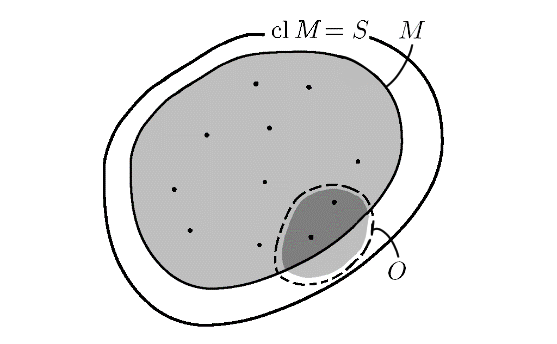
\includegraphics[width=94mm]{8.1.2.a.PNG}
\end{center}
\begin{proof}
位相空間$\left( S,\mathfrak{O} \right)$が与えられたとき、その集合$M$がその集合$S$において稠密であるなら、${\mathrm{cl}}M = S$が成り立つ。したがって、次のようになる。
\begin{align*}
\emptyset = S \setminus S = S \setminus {\mathrm{cl}}M = {\mathrm{int}}(S \setminus M)
\end{align*}
逆に、${\mathrm{int}}(S \setminus M) = \emptyset$が成り立つなら、開核と閉包の関係より${\mathrm{int}}(S \setminus M) = S \setminus {\mathrm{cl}}M$が成り立ち、したがって、${\mathrm{cl}}M = S$が成り立つ。\par
${\mathrm{cl}}M = S$が成り立つかつ、$\exists O \in \mathfrak{O \setminus}\left\{ \emptyset \right\}$に対し、$O \cap M = \emptyset$が成り立つと仮定すると、その集合$O$は空集合ではないので、その集合$M$は空集合であり、空集合は閉集合でもあるので、${\mathrm{cl}}M = {\mathrm{cl}}\emptyset = \emptyset$が成り立つが、これは$S = \emptyset$が成り立つことになり位相の定義に矛盾している。したがって、${\mathrm{cl}}M = S$が成り立つなら、$\forall O \in \mathfrak{O \setminus}\left\{ \emptyset \right\}$に対し、$O \cap M \neq \emptyset$が成り立つ。\par
逆に、${\mathrm{cl}}M \neq S$が成り立つなら、集合$S \setminus {\mathrm{cl}}M$は空集合ではないかつ、開集合となる。したがって、$S \setminus {\mathrm{cl}}M \cap {\mathrm{cl}}M = \emptyset$が成り立つ。ここで、$M \subseteq {\mathrm{cl}}M$が成り立つことに注意すれば、$S \setminus {\mathrm{cl}}M \cap M = \emptyset$も成り立つ。これにより、その集合$M$がその集合$S$において稠密でないなら、$\exists O \in \mathfrak{O \setminus}\left\{ \emptyset \right\}$に対し、$O \cap M = \emptyset$が成り立つことになる。対偶律より、$\forall O \in \mathfrak{O \setminus}\left\{ \emptyset \right\}$に対し、$O \cap M \neq \emptyset$が成り立つなら、その集合$M$はその集合$S$において稠密であることになる。
\end{proof}
\begin{dfn}
位相空間$\left( S,\mathfrak{O} \right)$において、その集合$S$において稠密であるかつ、たかだか可算集合である集合$M$が存在するとき、即ち、$\exists M \in \mathfrak{P}(S)$に対し、${\mathrm{cl}}M = S$が成り立つかつ、${\#}M \leq \aleph_{0}$が成り立つとき、その位相空間$\left( S,\mathfrak{O} \right)$は可分であるなどという。
\end{dfn}
\begin{thm}\label{8.1.2.20}
第2可算公理を満たす位相空間$\left( S,\mathfrak{O} \right)$は可分である。
\end{thm}
\begin{proof}
第2可算公理を満たす位相空間$\left( S,\mathfrak{O} \right)$が与えられたとき、たかだか可算集合であるその位相空間$\left( S,\mathfrak{O} \right)$の開基$\mathfrak{B}$が存在することになる。ここで、その集合$\mathfrak{B}$の元の族$\left\{ W_{\lambda} \right\}_{\lambda \in \varLambda}$が与えられたとき、その添数集合$\varLambda$を空集合とすれば、その和集合$\bigcup_{\lambda \in \varLambda} W_{\lambda}$は空集合となるので、集合$\mathfrak{B \setminus}\left\{ \emptyset \right\}$もその位相空間$\left( S,\mathfrak{O} \right)$の開基となる。ここで、$\forall\lambda \in \varLambda$に対し、選択の公理より$a_{\lambda} \in W_{\lambda}$なる元々$a_{\lambda}$を取り出し次式のように集合$M$が与えられれば、
\begin{align*}
M = \left\{ a_{\lambda} \in S \middle| \forall\lambda \in \varLambda\left[ a_{\lambda} \in W_{\lambda} \right] \right\}
\end{align*}
これはその集合$S$の部分集合となる。ここで、$\forall O \in \mathfrak{O}$に対し、開基の定義より$\exists\lambda \in \varLambda$に対し、$W_{\lambda} \subseteq O$が成り立つので、$a_{\lambda} \in O$が成り立つ。したがって、$a_{\lambda} \in O$かつ$a_{\lambda} \in M$が成り立つので、$O \cap M \neq \emptyset$が成り立つ。これが成り立つならそのときに限り、その集合$M$はその集合$S$において稠密となる。\par
ここで、その開基$\mathfrak{B}$はたかだか可算集合であるので、${\#}\mathfrak{B} \leq \aleph_{0}$が成り立つ。さらに、その集合$\mathfrak{B}$の元の族$\left\{ W_{\lambda} \right\}_{\lambda \in \varLambda}$が与えられているので、${\#}\varLambda \leq {\#}\mathfrak{B}$が成り立つかつ、次式のような写像$f$は明らかに全射であるので、
\begin{align*}
f:\varLambda \rightarrow M;\lambda \mapsto a_{\lambda}
\end{align*}
Bernsteinの定理よりその集合$M$からその集合$\varLambda$への単射が存在し${\#}M \leq {\#}\varLambda$が成り立つ。\par
以上より、${\#}M \leq {\#}\varLambda \leq {\#}\mathfrak{B} \leq \aleph_{0}$が成り立つので、その集合$M$もたかだか可算集合である。これにより、その位相空間$\left( S,\mathfrak{O} \right)$は可分である。
\end{proof}
\begin{thebibliography}{50}
\bibitem{1}
  松坂和夫, 集合・位相入門, 岩波書店, 1968. 新装版第2刷 p165-175 ISBN978-4-00-029871-1
\bibitem{2}
  加塩朋和. "一般位相A(2組)". 東京理科大学. \url{https://www.rs.tus.ac.jp/a25594/2018-2019_General_Topology.pdf} (2021-3-11 取得)
\bibitem{3}
  佃修一. "位相空間問題集". 琉球大学. \url{http://www.math.u-ryukyu.ac.jp/~tsukuda/lecturenotes/exercise-1104.pdf} (2021-3-29 取得)
\end{thebibliography}
\end{document}
